\documentclass[11pt,a4paper]{article}
\usepackage[margin=2cm]{geometry}
\usepackage{graphicx}
\usepackage{xcolor}
\usepackage{tcolorbox}
\usepackage{enumitem}
\usepackage{multicol}
\usepackage{amsmath}
\usepackage{amssymb}
\usepackage{fancyhdr}
\usepackage{hyperref}
\usepackage{tikz}
\usetikzlibrary{arrows.meta, positioning, shapes}

% Define colors
\definecolor{mlblue}{RGB}{31, 119, 180}
\definecolor{mlorange}{RGB}{255, 127, 14}
\definecolor{mlgreen}{RGB}{44, 160, 44}
\definecolor{mlred}{RGB}{214, 39, 40}
\definecolor{mlpurple}{RGB}{148, 103, 189}

% Header and footer
\pagestyle{fancy}
\fancyhf{}
\lhead{Week 1: Theory Discovery Tools}
\rhead{Clustering \& Innovation}
\cfoot{Page \thepage}

\title{\Large\textbf{Theory Discovery Tools}\\
\vspace{0.5em}
\large Building Your Own Clustering Theory - Week 1}
\author{BSc Machine Learning for Innovation\\
\textit{Discovery Cards \& Worksheets}}
\date{}

\begin{document}
\maketitle
\thispagestyle{fancy}

\begin{tcolorbox}[colback=mlgreen!10, colframe=mlgreen!50, title={\textbf{How to Use These Tools}}]
These cards and worksheets guide you through discovering clustering theory yourself. Cut out the cards, use them during exercises, and document your discoveries in the worksheets.
\end{tcolorbox}

% ============================================================
\section*{Part 1: Discovery Cards}
% ============================================================

\subsection*{Observation Cards}
Cut along dotted lines. Use these to guide your observations.

\begin{center}
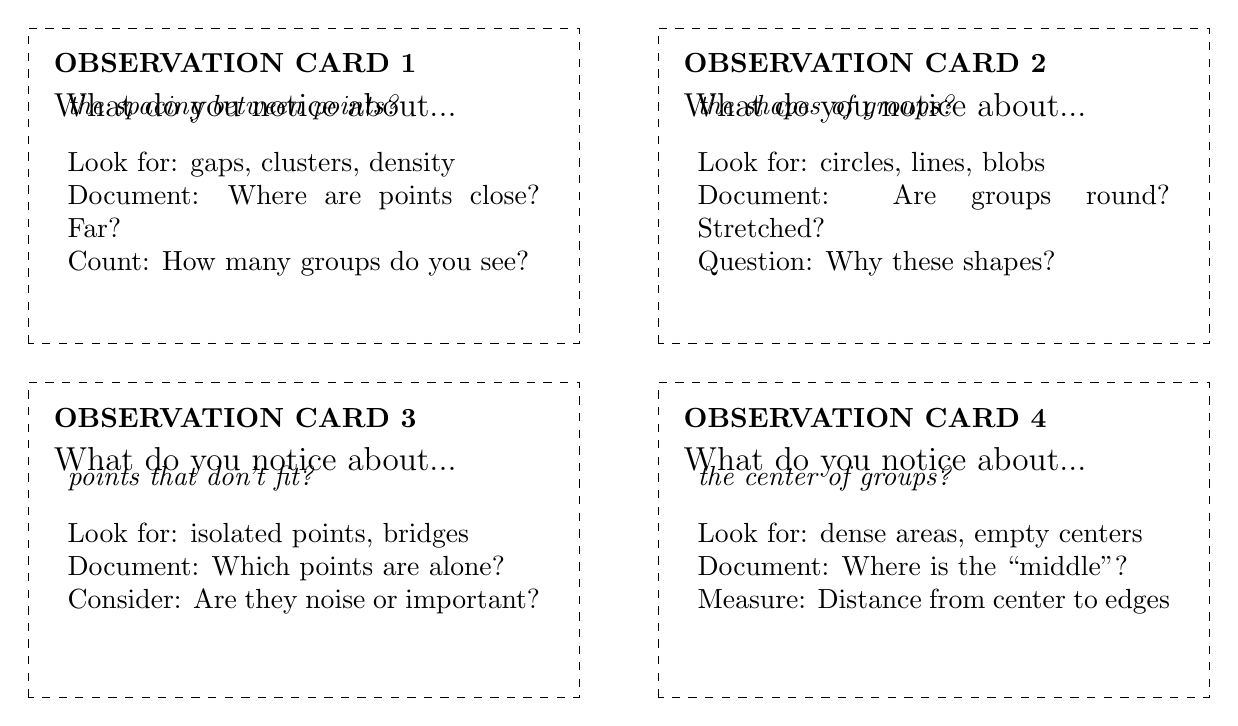
\begin{tikzpicture}
% Card 1
\draw[dashed] (0,0) rectangle (7,4);
\node[anchor=north west] at (0.2,3.8) {\textbf{OBSERVATION CARD 1}};
\node[anchor=north west] at (0.2,3.3) {\large What do you notice about...};
\node[anchor=center] at (3.5,2) {
\begin{minipage}{6cm}
\textit{the spacing between points?}\\[0.3cm]
Look for: gaps, clusters, density\\
Document: Where are points close? Far?\\
Count: How many groups do you see?
\end{minipage}
};

% Card 2
\draw[dashed] (8,0) rectangle (15,4);
\node[anchor=north west] at (8.2,3.8) {\textbf{OBSERVATION CARD 2}};
\node[anchor=north west] at (8.2,3.3) {\large What do you notice about...};
\node[anchor=center] at (11.5,2) {
\begin{minipage}{6cm}
\textit{the shapes of groups?}\\[0.3cm]
Look for: circles, lines, blobs\\
Document: Are groups round? Stretched?\\
Question: Why these shapes?
\end{minipage}
};

% Card 3
\draw[dashed] (0,-4.5) rectangle (7,-0.5);
\node[anchor=north west] at (0.2,-0.7) {\textbf{OBSERVATION CARD 3}};
\node[anchor=north west] at (0.2,-1.2) {\large What do you notice about...};
\node[anchor=center] at (3.5,-2.5) {
\begin{minipage}{6cm}
\textit{points that don't fit?}\\[0.3cm]
Look for: isolated points, bridges\\
Document: Which points are alone?\\
Consider: Are they noise or important?
\end{minipage}
};

% Card 4
\draw[dashed] (8,-4.5) rectangle (15,-0.5);
\node[anchor=north west] at (8.2,-0.7) {\textbf{OBSERVATION CARD 4}};
\node[anchor=north west] at (8.2,-1.2) {\large What do you notice about...};
\node[anchor=center] at (11.5,-2.5) {
\begin{minipage}{6cm}
\textit{the center of groups?}\\[0.3cm]
Look for: dense areas, empty centers\\
Document: Where is the ``middle''?\\
Measure: Distance from center to edges
\end{minipage}
};
\end{tikzpicture}
\end{center}

\newpage
\subsection*{Hypothesis Cards}
Use these to form theories about clustering.

\begin{center}
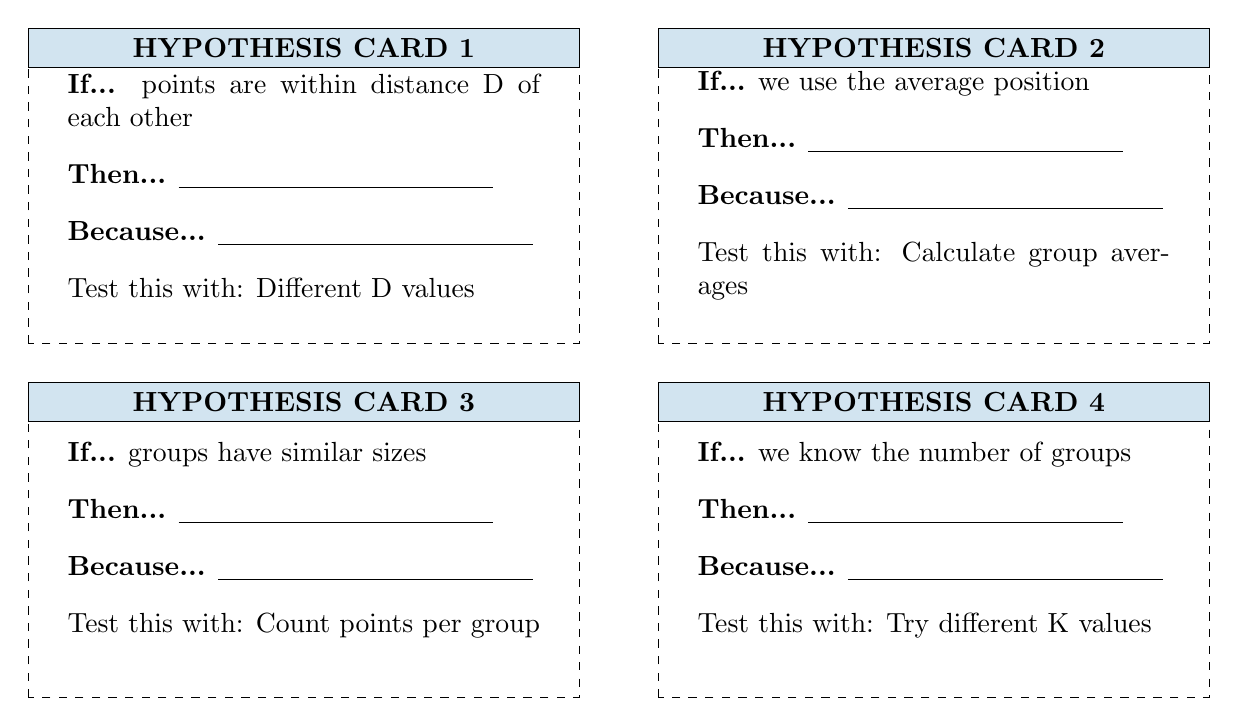
\begin{tikzpicture}
% Card 1
\draw[dashed] (0,0) rectangle (7,4);
\draw[fill=mlblue!20] (0,3.5) rectangle (7,4);
\node[anchor=center] at (3.5,3.75) {\textbf{HYPOTHESIS CARD 1}};
\node[anchor=center] at (3.5,2) {
\begin{minipage}{6cm}
\textbf{If...} points are within distance D of each other\\[0.3cm]
\textbf{Then...} \underline{\hspace{4cm}}\\[0.3cm]
\textbf{Because...} \underline{\hspace{4cm}}\\[0.3cm]
Test this with: Different D values
\end{minipage}
};

% Card 2
\draw[dashed] (8,0) rectangle (15,4);
\draw[fill=mlblue!20] (8,3.5) rectangle (15,4);
\node[anchor=center] at (11.5,3.75) {\textbf{HYPOTHESIS CARD 2}};
\node[anchor=center] at (11.5,2) {
\begin{minipage}{6cm}
\textbf{If...} we use the average position\\[0.3cm]
\textbf{Then...} \underline{\hspace{4cm}}\\[0.3cm]
\textbf{Because...} \underline{\hspace{4cm}}\\[0.3cm]
Test this with: Calculate group averages
\end{minipage}
};

% Card 3
\draw[dashed] (0,-4.5) rectangle (7,-0.5);
\draw[fill=mlblue!20] (0,-1) rectangle (7,-0.5);
\node[anchor=center] at (3.5,-0.75) {\textbf{HYPOTHESIS CARD 3}};
\node[anchor=center] at (3.5,-2.5) {
\begin{minipage}{6cm}
\textbf{If...} groups have similar sizes\\[0.3cm]
\textbf{Then...} \underline{\hspace{4cm}}\\[0.3cm]
\textbf{Because...} \underline{\hspace{4cm}}\\[0.3cm]
Test this with: Count points per group
\end{minipage}
};

% Card 4
\draw[dashed] (8,-4.5) rectangle (15,-0.5);
\draw[fill=mlblue!20] (8,-1) rectangle (15,-0.5);
\node[anchor=center] at (11.5,-0.75) {\textbf{HYPOTHESIS CARD 4}};
\node[anchor=center] at (11.5,-2.5) {
\begin{minipage}{6cm}
\textbf{If...} we know the number of groups\\[0.3cm]
\textbf{Then...} \underline{\hspace{4cm}}\\[0.3cm]
\textbf{Because...} \underline{\hspace{4cm}}\\[0.3cm]
Test this with: Try different K values
\end{minipage}
};
\end{tikzpicture}
\end{center}

\newpage
\subsection*{Test Cards}
Validate your theories with these experiments.

\begin{center}
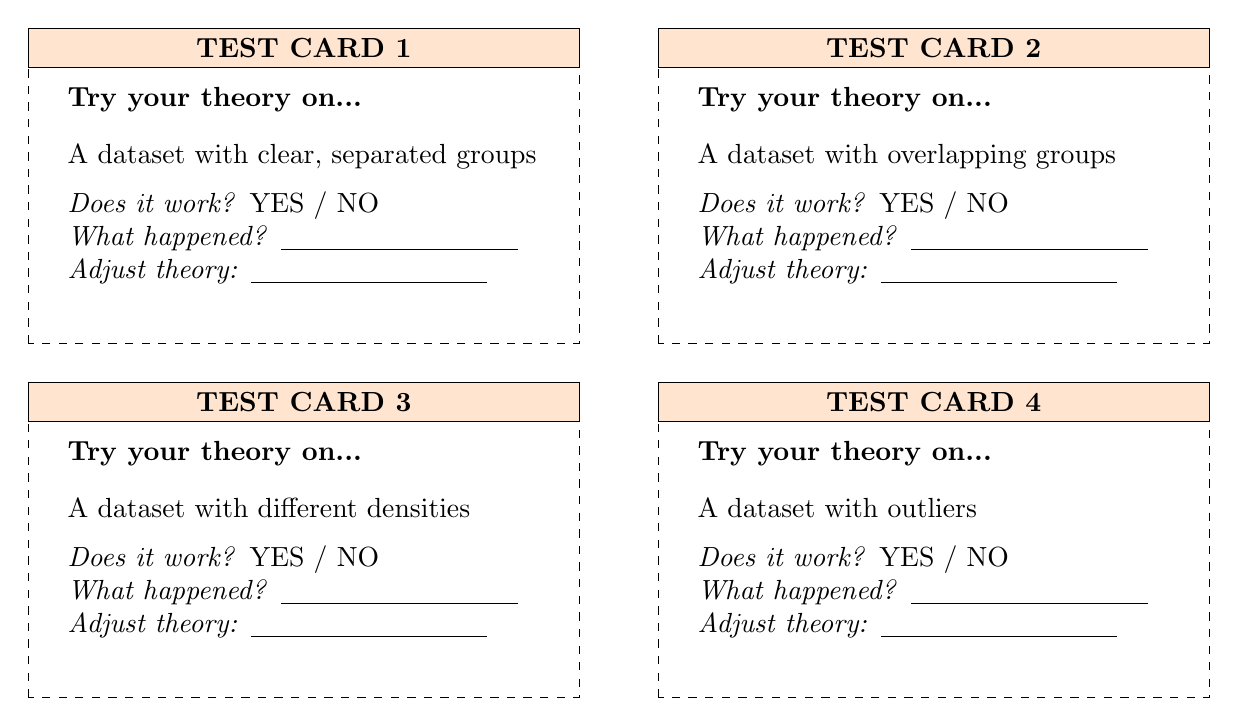
\begin{tikzpicture}
% Card 1
\draw[dashed] (0,0) rectangle (7,4);
\draw[fill=mlorange!20] (0,3.5) rectangle (7,4);
\node[anchor=center] at (3.5,3.75) {\textbf{TEST CARD 1}};
\node[anchor=center] at (3.5,2) {
\begin{minipage}{6cm}
\textbf{Try your theory on...}\\[0.3cm]
A dataset with clear, separated groups\\[0.2cm]
\textit{Does it work?} YES / NO\\
\textit{What happened?} \underline{\hspace{3cm}}\\
\textit{Adjust theory:} \underline{\hspace{3cm}}
\end{minipage}
};

% Card 2
\draw[dashed] (8,0) rectangle (15,4);
\draw[fill=mlorange!20] (8,3.5) rectangle (15,4);
\node[anchor=center] at (11.5,3.75) {\textbf{TEST CARD 2}};
\node[anchor=center] at (11.5,2) {
\begin{minipage}{6cm}
\textbf{Try your theory on...}\\[0.3cm]
A dataset with overlapping groups\\[0.2cm]
\textit{Does it work?} YES / NO\\
\textit{What happened?} \underline{\hspace{3cm}}\\
\textit{Adjust theory:} \underline{\hspace{3cm}}
\end{minipage}
};

% Card 3
\draw[dashed] (0,-4.5) rectangle (7,-0.5);
\draw[fill=mlorange!20] (0,-1) rectangle (7,-0.5);
\node[anchor=center] at (3.5,-0.75) {\textbf{TEST CARD 3}};
\node[anchor=center] at (3.5,-2.5) {
\begin{minipage}{6cm}
\textbf{Try your theory on...}\\[0.3cm]
A dataset with different densities\\[0.2cm]
\textit{Does it work?} YES / NO\\
\textit{What happened?} \underline{\hspace{3cm}}\\
\textit{Adjust theory:} \underline{\hspace{3cm}}
\end{minipage}
};

% Card 4
\draw[dashed] (8,-4.5) rectangle (15,-0.5);
\draw[fill=mlorange!20] (8,-1) rectangle (15,-0.5);
\node[anchor=center] at (11.5,-0.75) {\textbf{TEST CARD 4}};
\node[anchor=center] at (11.5,-2.5) {
\begin{minipage}{6cm}
\textbf{Try your theory on...}\\[0.3cm]
A dataset with outliers\\[0.2cm]
\textit{Does it work?} YES / NO\\
\textit{What happened?} \underline{\hspace{3cm}}\\
\textit{Adjust theory:} \underline{\hspace{3cm}}
\end{minipage}
};
\end{tikzpicture}
\end{center}

\newpage
\subsection*{Reflection Cards}
Understand why your discoveries work.

\begin{center}
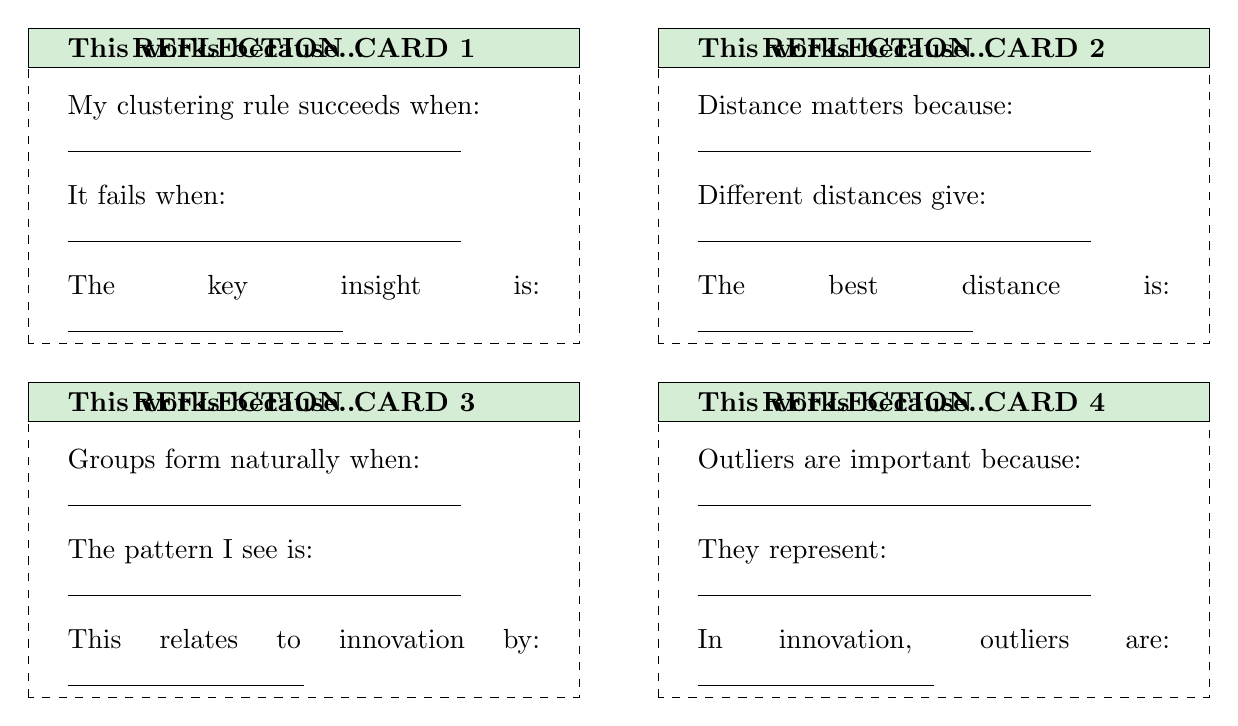
\begin{tikzpicture}
% Card 1
\draw[dashed] (0,0) rectangle (7,4);
\draw[fill=mlgreen!20] (0,3.5) rectangle (7,4);
\node[anchor=center] at (3.5,3.75) {\textbf{REFLECTION CARD 1}};
\node[anchor=center] at (3.5,2) {
\begin{minipage}{6cm}
\textbf{This works because...}\\[0.3cm]
My clustering rule succeeds when:\\
\underline{\hspace{5cm}}\\[0.3cm]
It fails when:\\
\underline{\hspace{5cm}}\\[0.3cm]
The key insight is: \underline{\hspace{3.5cm}}
\end{minipage}
};

% Card 2
\draw[dashed] (8,0) rectangle (15,4);
\draw[fill=mlgreen!20] (8,3.5) rectangle (15,4);
\node[anchor=center] at (11.5,3.75) {\textbf{REFLECTION CARD 2}};
\node[anchor=center] at (11.5,2) {
\begin{minipage}{6cm}
\textbf{This works because...}\\[0.3cm]
Distance matters because:\\
\underline{\hspace{5cm}}\\[0.3cm]
Different distances give:\\
\underline{\hspace{5cm}}\\[0.3cm]
The best distance is: \underline{\hspace{3.5cm}}
\end{minipage}
};

% Card 3
\draw[dashed] (0,-4.5) rectangle (7,-0.5);
\draw[fill=mlgreen!20] (0,-1) rectangle (7,-0.5);
\node[anchor=center] at (3.5,-0.75) {\textbf{REFLECTION CARD 3}};
\node[anchor=center] at (3.5,-2.5) {
\begin{minipage}{6cm}
\textbf{This works because...}\\[0.3cm]
Groups form naturally when:\\
\underline{\hspace{5cm}}\\[0.3cm]
The pattern I see is:\\
\underline{\hspace{5cm}}\\[0.3cm]
This relates to innovation by: \underline{\hspace{3cm}}
\end{minipage}
};

% Card 4
\draw[dashed] (8,-4.5) rectangle (15,-0.5);
\draw[fill=mlgreen!20] (8,-1) rectangle (15,-0.5);
\node[anchor=center] at (11.5,-0.75) {\textbf{REFLECTION CARD 4}};
\node[anchor=center] at (11.5,-2.5) {
\begin{minipage}{6cm}
\textbf{This works because...}\\[0.3cm]
Outliers are important because:\\
\underline{\hspace{5cm}}\\[0.3cm]
They represent:\\
\underline{\hspace{5cm}}\\[0.3cm]
In innovation, outliers are: \underline{\hspace{3cm}}
\end{minipage}
};
\end{tikzpicture}
\end{center}

\newpage
% ============================================================
\section*{Part 2: Theory Building Worksheets}
% ============================================================

\subsection*{Worksheet 1: Rule Creator}
\textit{Template for writing clustering rules}

\begin{tcolorbox}[colback=white, colframe=mlpurple!50, title={\textbf{Create Your Clustering Algorithm}}]

\textbf{Step 1: Define ``Belongs Together''}\\[0.2cm]
Two points belong in the same group if:\\
\underline{\hspace{12cm}}\\
\underline{\hspace{12cm}}\\[0.5cm]

\textbf{Step 2: Write Your Algorithm}\\[0.2cm]
\begin{enumerate}
\item Start with: \underline{\hspace{10cm}}
\item For each point: \underline{\hspace{9.5cm}}
\item Calculate: \underline{\hspace{10cm}}
\item Assign to group if: \underline{\hspace{9cm}}
\item Repeat until: \underline{\hspace{9.5cm}}
\item Stop when: \underline{\hspace{10cm}}
\end{enumerate}

\textbf{Step 3: Handle Special Cases}\\[0.2cm]
If a point doesn't fit any group: \underline{\hspace{8cm}}\\
If groups overlap: \underline{\hspace{10cm}}\\
If I don't know K: \underline{\hspace{10cm}}\\[0.5cm]

\textbf{Step 4: Name Your Algorithm}\\[0.2cm]
My clustering algorithm is called: \underline{\hspace{8cm}}\\
Because it: \underline{\hspace{11cm}}

\end{tcolorbox}

\newpage
\subsection*{Worksheet 2: Pattern Finder}
\textit{Guide for identifying regularities}

\begin{tcolorbox}[colback=white, colframe=mlblue!50, title={\textbf{Finding Patterns in Data}}]

\textbf{Visual Pattern Recognition}\\[0.2cm]
\begin{center}
\begin{tabular}{|l|c|c|c|}
\hline
\textbf{Pattern Type} & \textbf{I See This} & \textbf{It Means} & \textbf{Algorithm Needed} \\
\hline
Circular groups & YES / NO & & \\[0.5cm]
\hline
Elongated groups & YES / NO & & \\[0.5cm]
\hline
Nested groups & YES / NO & & \\[0.5cm]
\hline
Chain connections & YES / NO & & \\[0.5cm]
\hline
Varying density & YES / NO & & \\[0.5cm]
\hline
Clear outliers & YES / NO & & \\[0.5cm]
\hline
\end{tabular}
\end{center}

\textbf{Numerical Pattern Recognition}\\[0.2cm]
When I count groups at different scales:\\
- Fine scale (small distance): \underline{\hspace{2cm}} groups\\
- Medium scale: \underline{\hspace{2cm}} groups\\
- Coarse scale (large distance): \underline{\hspace{2cm}} groups\\[0.3cm]

The pattern is: \underline{\hspace{10cm}}\\[0.5cm]

\textbf{Innovation Pattern Recognition}\\[0.2cm]
In my field, natural groups form around:\\
\begin{itemize}
\item \underline{\hspace{10cm}}
\item \underline{\hspace{10cm}}
\item \underline{\hspace{10cm}}
\end{itemize}

These patterns suggest the clustering approach: \underline{\hspace{7cm}}

\end{tcolorbox}

\newpage
\subsection*{Worksheet 3: Theory Tester}
\textit{Framework for validation}

\begin{tcolorbox}[colback=white, colframe=mlorange!50, title={\textbf{Testing Your Clustering Theory}}]

\textbf{Theory Statement}\\
My theory: \underline{\hspace{11cm}}\\
\underline{\hspace{12cm}}\\[0.5cm]

\textbf{Prediction Table}\\
\begin{center}
\begin{tabular}{|l|l|l|}
\hline
\textbf{If my theory is correct...} & \textbf{I expect to see...} & \textbf{Actually saw...} \\
\hline
On dataset A: & & \\[1cm]
\hline
On dataset B: & & \\[1cm]
\hline
On dataset C: & & \\[1cm]
\hline
\end{tabular}
\end{center}

\textbf{Success Metrics}\\
My clustering is good when:\\
\begin{itemize}
\item Within-cluster distance is: \underline{\hspace{7cm}}
\item Between-cluster distance is: \underline{\hspace{7cm}}
\item Number of outliers is: \underline{\hspace{8cm}}
\item Groups are balanced: YES / NO / SOMETIMES
\end{itemize}

\textbf{Theory Refinement}\\
What worked: \underline{\hspace{10cm}}\\
What failed: \underline{\hspace{10cm}}\\
Revised theory: \underline{\hspace{10cm}}\\
\underline{\hspace{12cm}}

\end{tcolorbox}

\newpage
\subsection*{Worksheet 4: Concept Connector}
\textit{Linking discoveries to formal terms}

\begin{tcolorbox}[colback=white, colframe=mlgreen!50, title={\textbf{From Your Words to Formal Theory}}]

\textbf{Translation Table}\\
Connect what you discovered to the formal terminology:

\begin{center}
\begin{tabular}{|p{4cm}|p{4cm}|p{4cm}|}
\hline
\textbf{What I Called It} & \textbf{Formal Term} & \textbf{Why It's Important} \\
\hline
``Group middle point'' & Centroid & Represents the cluster \\
\hline
``How spread out'' & & \\[0.7cm]
\hline
``Doesn't fit anywhere'' & & \\[0.7cm]
\hline
``How tight the group is'' & & \\[0.7cm]
\hline
``Space between groups'' & & \\[0.7cm]
\hline
``Best number of groups'' & & \\[0.7cm]
\hline
\end{tabular}
\end{center}

\textbf{Algorithm Matching}\\
My approach is most similar to:\\
\begin{itemize}
\item[$\square$] K-means (uses centers, equal groups)
\item[$\square$] DBSCAN (uses density, finds shapes)
\item[$\square$] Hierarchical (builds tree, multiple scales)
\item[$\square$] GMM (uses probability, overlapping groups)
\item[$\square$] Something new: \underline{\hspace{6cm}}
\end{itemize}

\textbf{Innovation Applications}\\
My clustering discovery applies to innovation by:\\
\begin{enumerate}
\item \underline{\hspace{11cm}}
\item \underline{\hspace{11cm}}
\item \underline{\hspace{11cm}}
\end{enumerate}

\textbf{Key Insight}\\
The most important thing I learned about clustering is:\\
\underline{\hspace{12cm}}\\
\underline{\hspace{12cm}}

\end{tcolorbox}

\end{document}